\section{Integrazione rispetto alla probabilità}
Come osservato nei capitoli precedenti, una variabile aleatoria può assumere diversi valori con determinate probabilità.
Il \emph{valore atteso} è, in buona sostanza, la media di tutti i valori che una variabile aleatoria reale può assumere, ciascuno pesato per la sua probabilità di comparire.
A partire da questo capitolo costruiremo la \emph{regola del valore atteso} cominciando da casi elementari, le variabili \emph{semplici}, per arrivare a casi via via più complessi e generici, ma sempre tenendo come riferimento il concetto di valore atteso sopra illustrato.
Saranno inoltre sviluppate le utilissime proprietà del valore atteso, che assumeranno crescente importanza nel proseguimento del corso, e di un altro indicatore strettamente collegato al valore atteso, la \emph{varianza}, che descrive l'ampiezza della distribuzione intorno alla media.
\smallskip

\begin{defn}
	\index{variabile aleatoria!reale}
	Una variabile aleatoria a valori reali $X:\Omega \to \RR$ si dice \textbf{variabile aleatoria reale} (d'ora in avanti \textbf{VAR}).
\end{defn}
Ovviamente solo una variabile aleatoria a valori numerici (reali nel caso più generale) può ammettere una media sui valori del codominio.
\smallskip

\begin{defn}
	\index{valore atteso}
	\index{integrale (valore atteso)}
	\index{media!(valore atteso)}
	Siano dati uno spazio di probabilità $\Dom$, una VA $X:\Omega \to \RR$ e una legge $P^X$ su $\Bc$.
	Si definisca $\EE[X]$ (talvolta scritto $\mu$), \textbf{valore atteso} di $X$, o \textbf{integrale} di $X$, come il valore centrale rispetto ai possibili esiti $X(\omega)$ di $X$, ovvero una media pesata dei possibili valori di $X(\omega) \enspace \forall \omega \in \Omega$.
	Per il valore atteso saranno utilizzate le seguenti scritture equivalenti:
	$$
  		\EE[X] = \int_\Omega X(\omega) \, \PP(\de \omega) = \int_\Omega X(\omega) \, \dPP(\omega) = \int_\Omega X \, \dPP
	$$
\end{defn}

\subsection{Variabili aleatorie semplici}
\begin{defn}
  \index{variabile aleatoria!semplice}
  Una VAR $X$ è detta \textbf{semplice} se può assumere solo un numero finito di valori, ovvero se  $\#\im(X) = n < +\infty$ (con $n \in \NN$).
\end{defn}

\medskip
\begin{prop}[criterio per VAR semplici]
  $X:\Omega \to \RR$ è una VAR semplice se e solo se:
  $$X = \sum\limits_{k=1}^{n} x_k \Ind_{A_k}, \quad
  \text{con } A_k = (X = x_k) \in \Ac \enspace \forall k = 1,\dots,n$$
\end{prop}
Il criterio dà una formula di ``scomposizione'' universale per tutte le VA semplici. \\*
Come è possibile evincere dalla figura \ref{fig-var-semplice-dom}, gli $A_k$ sono disgiunti (ovvero tali che $A_k \cap A_l = \varnothing \ \forall k \neq l$) e coprono l'intero dominio $\left(\bigcup\limits_{k=1}^{n} A_k = \Omega\right)$, ovvero la collezione $\{A_k\}$ è una partizione\footnote{In realtà nella definizione di partizione è richiesto che tutti gli insiemi devono avere probabilità non nulla, mentre qui non necessariamente $\PP(A_k) > 0 \, \forall k$; tuttavia questa precisazione non ha particolare importanza nel caso in esame.}.
Si ha dunque che:
$$X(\omega) = \sum\limits_{k=1}^{n} x_k \Ind_{A_k}(\omega) =
\begin{cases}
  x_1 &  \omega \in A_1\\
  x_2 &  \omega \in A_2\\
  \dots & \dots \\
  x_n &  \omega \in A_n
\end{cases}$$
Questa è una ``\emph{finta sommatoria}'', nel senso che per ogni $\omega$ una sola delle indicatrici vale 1, e quindi un solo elemento della sommatoria alla volta è non nullo.
In questo caso, inoltre, tutte le controimmagini sono misurabili.

\begin{figure}[H]
  \centering
  \def\drect {(-1.5, -1.5) rectangle (3, 1.5)}
  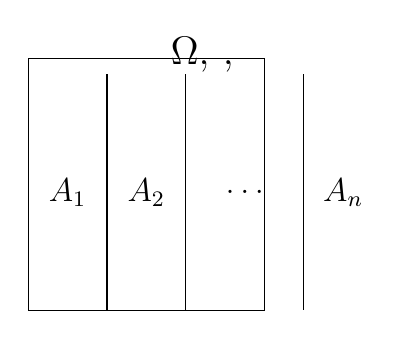
\begin{tikzpicture}
    \draw \drect;
    \draw(-0.5,1.5) -- (-0.5,-1.5);
    \draw(0.5,1.5) -- (0.5,-1.5);
    \draw(2,1.5) -- (2,-1.5);
    %Scritte
    \node at (0.75, 1.75) {\Large $\Omega, \, \Ac, \, \PP$};
    \node at (-1, 0) {\large $A_1$};
    \node at (0, 0) {\large $A_2$};
    \node at (1.25, 0) {\large $\dots$};
    \node at (2.5, 0) {\large $A_n$};
  \end{tikzpicture}
  \caption{dominio di una VAR semplice}
  \label{fig-var-semplice-dom}
\end{figure}

\begin{dimo}
\textbf{($\implies$)}: $X = \sum\limits_{k=1}^{n} x_k \Ind_{(X = x_k)}$ perché $\im(X) = \{x_1, \, \dots, \, x_n\}$. \\*
\textbf{($\impliedby$)}:
\begin{enumerate}
  \item $X$ è reale perché $x_k \in \RR \ \forall k$;
  \item $X$ è semplice perché $\#\im(X) = n \in \NN$;
  \item $X$ è misurabile perché le indicatrici sono misurabili e il prodotto di quantità misurabili è misurabile. \qedhere
\end{enumerate}
\end{dimo}

\smallskip
\begin{nb}
    Sia $\{\widetilde A_i\}$ una collezione di cardinalità $n$ di insiemi generici appartenenti ad $\Ac$ e siano $a_i \in \RR \, \forall i$.
    A differenza dell'esempio precedente, non chiediamo che gli $\widetilde A_i$ siano disgiunti né che $\bigcup_i \widetilde A_i = \Omega$. \\
    Definiamo ora $X = \sum\limits_{i = 1}^{v} a_i \Ind_{\widetilde A_i}$,    dove $v < +\infty$ è il numero (arbitrario e non necessariamente uguale a $n$) di elementi sommati.
    Allora $X$ è una VAR semplice, perché $\#\im(X) < +\infty$: essendo $v$ un numero finito, la cardinalità dell'immagine non può essere infinita.
\end{nb}

\smallskip
\begin{ese}
  Presa la VAR sopra definita, e dato un dominio di cardinalità $v = 2$, i possibili valori della VAR sono 4.
  In generale, l'immagine ha cardinalità $2^v < +\infty$ casi.\footnote{Questo è vero in quanto
	``esistono due casi per ogni insieme: appartenenza e non appartenenza'' -Capitan Findus}

  \begin{figure}[H]
    \centering
    \def\firstcircle{(0,0) circle (1.2cm)}
    \def\secondcircle{(-35:1.5cm) circle (1.2cm)}
    \def\drect {(-1.5,-2.5) rectangle (3,1.7)}
    \begin{tikzpicture}
      \begin{scope}[fill opacity=0.5]
        \fill[lightblue] \firstcircle;
        \fill[darkgreen] \secondcircle;
        \draw \firstcircle;
        \draw \secondcircle;
      \end{scope}
      \draw \drect node[below left] {\Large $\Omega, \, \Ac, \, \PP$};
      \node at (-.3,.3) {\huge $A_1$};
      \node at (1.5,-1.2) {\huge $A_2$};

      %Frecce
      \draw[->, line width=0.30mm] (3.3,-0.4) node[above,xshift=1.5cm] {\Large $X$} -- (6.3,-0.4);
      \draw[->, line width=0.60mm] (7,-1.8) node[below, yshift=-.3cm] {\Large $\RR, \Bc$} -- (7,1.7);
      %Tacchette
      \draw[line width=0.50mm] (7.2,-1.2) node[right] {\large $A_1$} -- (6.8, -1.2);
      \draw[line width=0.50mm] (7.2,-0.1) node[right] {\large $A_1 + A_2$} -- (6.8, -0.1);
      \draw[line width=0.50mm] (7.2,0.5) node[right] {\large $0$} -- (6.8, 0.5);
      \draw[line width=0.50mm] (7.2,1) node[right] {\large $A_2$} -- (6.8, 1);
      %Pallini
      \node at (-0.6 ,-1.6) {\textbullet};
      \node at (-0.4,-0.7) {\textbullet};
      \node at (0.4,-0.6) {\textbullet};
      \node at (0.8,-1.3) {\textbullet};
    \end{tikzpicture}
    \caption{VAR semplice con cardinalità 2}
    \label{VAR_semplice_val}
  \end{figure}
\end{ese}

\subsection{Integrazione di variabili aleatorie reali}
\subsubsection{Variabili semplici}
\begin{defn}\label{defn-valore-atteso-semplici}
  \index{valore atteso!per VAR semplici}
  Data $X = \sum\limits_{k=1}^{n} x_k \Ind_{(X = x_k)}$ VAR semplice definita sul dominio $\Omega$, si dice \textbf{valore atteso} di $X$ la seguente quantità:
  $$\EE[X] = \int_{\Omega} X \, \dPP \coloneqq \sum\limits_{k=1}^{n} x_k \, \PP(X = x_k)$$
\end{defn}
Nel caso delle VA semplici, l'integrale è formato solo da un numero finito di casi, quindi si trasforma in una sommatoria.
Si osservi la figura \ref{Valore_atteso_VAR_semplice}.
Ogni evento $A_k$ ha la sua probabilità di verificarsi, rappresentata dalle aree dei rispettivi rettangoli.
La VA $X$ assegna un valore reale ad ognuno di questi eventi.
Il valore atteso di $X$ è semplicemente la media di questi valori, pesati rispetto alle probabilità dei corrispondenti eventi.
\begin{figure}[H]
  \centering
  \def\drect {(-1.5, -1.5) rectangle (2.5, 1.5)}
  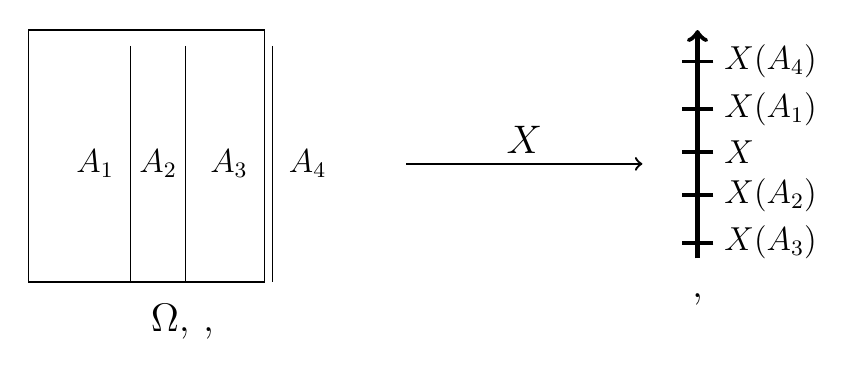
\begin{tikzpicture}
    \draw \drect;
    \draw(-0.2,1.5) -- (-0.2,-1.5);
    \draw(0.5,1.5) -- (0.5,-1.5);
    \draw(1.6,1.5) -- (1.6,-1.5);
    %Scritte
    \node at (0.5, -2) {\Large $\Omega, \, \Ac, \, \PP$};
    \node at (-0.6 5, 0) {\large $A_1$};
    \node at (0.15, 0) {\large $A_2$};
    \node at (1.05, 0) {\large $A_3$};
    \node at (2.05, 0) {\large $A_4$};

    %Frecce
    \draw[->, line width=0.30mm] (3.3,0) node[above,xshift=1.5cm] {\Large $X$} -- (6.3,0);
    \draw[->, line width=0.60mm] (7,-1.2) node[below, yshift=-.3cm] {\Large $\RR, \Bc$} -- (7,1.7);
    %Tacchette
    \draw[line width=0.50mm] (7.2,-1) node[right] {\large $X(A_3)$} -- (6.8, -1);
    \draw[line width=0.50mm] (7.2,-0.4) node[right] {\large $X(A_2)$} -- (6.8, -0.4);
    \draw[line width=0.50mm] (7.2,0.15) node[right] {\large $\Ex{X}$} -- (6.8, 0.15);
    \draw[line width=0.50mm] (7.2,0.7) node[right] {\large $X(A_1)$} -- (6.8, 0.7);
    \draw[line width=0.50mm] (7.2,1.3) node[right] {\large $X(A_4)$} -- (6.8, 1.3);
  \end{tikzpicture}
  \caption{valore atteso per una VAR semplice}
  \label{Valore_atteso_VAR_semplice}
\end{figure}
\begin{propb}\label{prop-valore-atteso-semplici}
  Siano $X$, $Y$ VAR semplici su $\Dom$ e sia $a \in \RR$. Allora:
  \begin{enumerate}
    \item $aX$ è una VAR semplice
    \item $\EE[aX] = a \EE[X]$
    \item $X = \sum\limits_{i=1}^{v} a_i \Ind_{\widetilde A_i}, \; \widetilde A_i \in \Ac \ \forall i
      \implies \EE[X] = \sum\limits_{i=1}^{v} a_i \PP(\widetilde A_i)$
    \item $X + Y$ è una VAR semplice
    \item $\EE[X+Y] = \EE[X] + \EE[Y]$
    \item $X \leq Y \; \forall \omega \in \Omega \implies \EE[X] \leq \EE[Y]$
  \end{enumerate}
\end{propb}
Le proprietà (2) e (5) dimostrano la linearità del valore atteso, e la (6) ne dimostra la positività.

\begin{dimo}
  \Fixvmode
  \begin{enumerate}
    \item È immediata, definendo la nuova VA $Y = aX = \sum\limits_{k = 1}^{n} (aX_k) \Ind_{A_k}$.\\*

      Si noti che $A_k = (X = x_k) = (Y = ax_k) \ \forall a \neq 0$.\\*
      $\Omega$ in $\PP(\Omega)$ è l'unica controimmagine possibile, infatti tutti gli elementi $\omega$ sono mappati in zero perché è l'unico valore che $Y$ può assumere.
      %?????????????? (Br1)
    \item Nel caso di $a = 0$ allora $Y = 0 \cdot X = 0$, quindi $\EE[Y] = 0 \cdot \PP(\Omega) = 0 = 0 \cdot \EE[X]$.\\*
      Nel caso generale di $a \neq 0$ si ha invece che:
      $$\EE[Y] = \EE[aX] = \sum\limits_{k=1}^{n} ax_k \PP(aX = ax_k) = a\sum\limits_{k=1}^n  x_k \PP(x = x_k) = a \EE[X]$$
      La tesi è dunque valida $\forall a \in \RR$.
    \item Si ponga $v = 2$ per semplicità di notazione (la dimostrazione del caso generale si svolge in modo simile).\\*
    È possibile definire esplicitamente $X$ VAR semplice bidimensionale nel seguente modo:
    $$X = \sum\limits_{i=1}^{2} a_i \Ind_{\widetilde A_i} = a_1 \Ind_{\widetilde A_1 \, \setminus \, \widetilde A_2} + a_2 \Ind_{\widetilde A_2 \, \setminus \, \widetilde A_1} + (a_1 + a_2) \Ind_{\widetilde A_1 \cap \widetilde A_2} + 0 \cdot \Ind_{(\widetilde A_1 \cup \widetilde A_2)^C}$$
    Infatti i quattro valori combinati linearmente sono gli unici valori che $X$ può assumere, e i quattro insiemi delle indicatrici formano una partizione per $\Omega$.
    Si delineano insomma quattro casi, come illustrato nell'esempio precedente con la figura \ref{VAR_semplice_val}:
    \begin{align*}
      \EE[X] &= a_1 \PP(\widetilde A_1 \ \setminus \ \widetilde A_2) + a_2  \PP(\widetilde A_2 \ \setminus \ \widetilde A_1) + (a_1 + a_2) \PP(\widetilde A_1, \widetilde A_2)\\
      &= a_1(\PP(\widetilde A_1 \ \setminus \ \widetilde A_2) + \PP(\widetilde A_1, \widetilde A_2)) + a_2(\PP(\widetilde A_2 \ \setminus \ \widetilde A_1) + \PP(\widetilde A_1, \widetilde A_2))\\
      &= a_1 \PP(\widetilde A_1) + a_2 \PP(\widetilde A_2)
    \end{align*}
    \item Essendo $X$ e $Y$ VAR, la loro somma è misurabile e semplice (vedi teorema \ref{teo-va-mis}).
    \item Scomponendo $X$ e $Y$ come ``finte sommatorie'' si ottiene:
      $$\EE[X+Y] = \EE \left[\sum\limits_{k=1}^n x_k \Ind_{(X = x_k)} + \sum\limits_{l=1}^m y_l \Ind_{(Y = y_l)} \right]$$
      Partizioniamo ora $\Omega$ regolarmente lungo $X$ e $Y$:
      \begin{figure}[H]
        \centering
        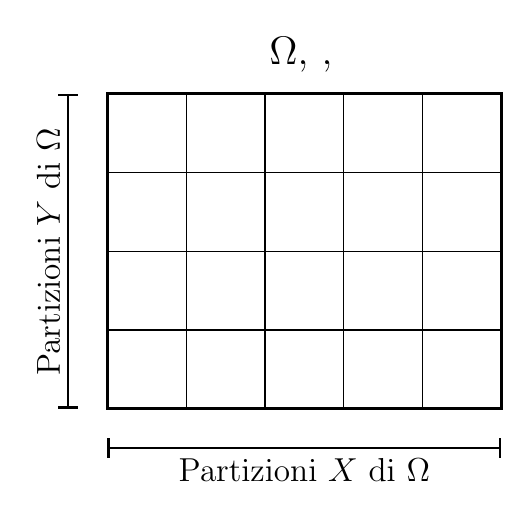
\begin{tikzpicture}
          \draw[scale=1] (0, 0) grid (5,4);
          \draw[very thick] (0, 0) rectangle (5, 4);
          %Scritte
          \node at (2.5,4.5) {\Large $\Omega, \, \Ac, \, \PP$};
          \draw[|-|, line width=0.30mm] (0, -0.5) node[below,xshift=2.5cm] {\large Partizioni $X$ di $\Omega$} -- (5, -0.5);
          \draw[|-|, line width=0.30mm] (-0.5, 0) node[left,yshift=3.70cm,xshift=-.25cm,rotate=90] {\large Partizioni $Y$ di $\Omega$} -- (-0.5, 4);
        \end{tikzpicture}
        \label{Partizioni_XY}
      \end{figure}
      Si verifica facilmente che il risultato ottenuto ha la seguente formulazione equivalente:
      \begin{align*}
        \EE[X+Y] &= \EE\left[\sum\limits_{k=1}^n \sum\limits_{l=1}^m (x_k+y_l) \Ind_{(X = x_k, Y = y_l)}\right] =\\
        & \text{(applicando il punto (3))} \\
        &= \sum\limits_{k=1}^n \sum\limits_{l=1}^m (x_k+y_l) \PP(X = x_k, Y = y_l) = \\
        &= \sum\limits_{k=1}^n \left[ x_k \sum\limits_{l=1}^m \PP(X = x_k, Y = y_l) \right] + \sum\limits_{l=1}^m \left[ y_l \sum\limits_{k=1}^n \PP(X = x_k, Y = y_l) \right] =\\
        &\text{(per le probabilità totali)}\\
        &= \sum\limits_{k=1}^n \left[ x_k \PP(X = x_k) \right] + \sum\limits_{l=1}^m \left[ y_l \PP(Y = y_l) \right] = \\
        &= \EE[X] + \EE[Y]
      \end{align*}
    \item Siano $X$ e $Y$ due VAR semplici così espresse:
      $$X = \sum\limits_{k=1}^{n} x_k \Ind_{(X = x_k)}, \quad Y = \sum\limits_{l=1}^{n} y_l \Ind_{(Y = y_l)}$$
      %prima c'era x_k \cap x_l \neq \varnothing, che cappero volesse dire non saprei ?.? Spero che ora sia giusto (Br1)
      %Per ipotesi $X \leq Y$, quindi vale la condizione $x_k \leq y_l$ in tutte le intersezioni della forma $(X = x_k) \cap (Y = y_l) \neq \varnothing$.
      %Mi spiace, è stato bello (Br2)
      Si noti che non è detto che $x_k \leq y_l \, \forall k,l$, perché i valori $x_k$ e $y_l$ non sono necessariamente definiti sulla stessa parte del dominio.
      Ad esempio nel caso raffigurato la partizione che ha immagine $x_3$ non deve essere minore di tutte le altre, bensì è sufficiente che valga $x_3 \leq y_2, y_3$.
      Questo è simile a quanto succede per una normale coppia di funzioni: il fatto che una funzione sia maggiore di un'altra non vuol dire necessariamente che, preso un qualsiasi valore della prima, esso sarà maggiore di \emph{tutti} i valori della seconda;
      il confronto avviene solo sulle coppie di valori che sono mappati dalla stessa parte di dominio.
      \begin{figure}[H]
        \centering
        \def\drect {(-1.5, -1.5) rectangle (2.5, 1.5)}
        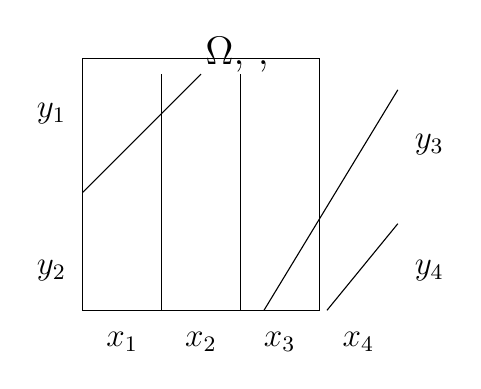
\begin{tikzpicture}
          \draw \drect;
          \draw(-0.5,1.5) -- (-0.5,-1.5);
          \draw(0.5,1.5) -- (0.5,-1.5);
          \draw(1.5,1.5) -- (1.5,-1.5);

          \draw(-1.5,0) -- (0,1.5);
          \draw(0.8,-1.5) -- (2.5,1.3);
          \draw(1.6,-1.5) -- (2.5,-0.4);
          %Scritte
          \node at (0.5, 1.75) {\Large $\Omega, \, \Ac, \, \PP$};
          \node at (-1, -1.9) {\large $x_1$};
          \node at (0, -1.9) {\large $x_2$};
          \node at (1, -1.9) {\large $x_3$};
          \node at (2, -1.9) {\large $x_4$};

          \node at (-1.9, 1) {\large $y_1$};
          \node at (-1.9, -1) {\large $y_2$};
          \node at (2.9, 0.6) {\large $y_3$};
          \node at (2.9, -1) {\large $y_4$};
        \end{tikzpicture}
        \label{Partizioni_XY_irr}
      \end{figure}
      Bisogna quindi creare una \emph{partizione comune} $\{\widetilde A_j\}$ per $X$ e $Y$ composta da tutte le intersezioni delle due partizioni precedenti.
      In altre parole, prendiamo la collezione $\{\widetilde A_j\}$ tale che:
      \begin{itemize}
      	\item $\widetilde A_j \in \Ac \, \forall j$
      	\item $\bigcup_j \widetilde A_j = \Omega$
      	\item $\widetilde A_j \cap \widetilde A_i = \varnothing \ \forall j \neq i$.
      \end{itemize}
      Ora si può dunque ripartizionare le VA $X$ e $Y$ sui nuovi $\widetilde A$:
      $$X = \sum\limits_{j} a_j \Ind_{\widetilde A_j}, \ \ Y = \sum\limits_j b_j \Ind_{\widetilde A_j}$$
      Poiché con l'introduzione della partizione comune gli insiemi delle indicatrici sono gli stessi per entrambe le VA, è finalmente possibile confrontare i valori delle VA su ogni pezzo di dominio.
      In particolare, possiamo affermare che $a_j \leq b_j \ \forall j$.
      Passando ai valori attesi:
      $$\EE[X] = \sum\limits_j a_j \PP(\widetilde A_j) \leq \sum\limits_{j} b_j \PP(\widetilde A_j) = \EE[Y] \qedhere$$
	\end{enumerate}
\end{dimo}

\subsubsection{Variabili positive}
Si vuole ora estendere il concetto di valore atteso dalle VA semplici a quelle che possono assumere ogni possibile valore su $\RR$, o comunque su insiemi di cardinalità infinita. \\*
Partiamo dalla trattazione per VA a valori positivi\footnote{La nomenclatura tecnicamente corretta sarebbe ``non negativi'', in quanto lo zero può essere incluso nel codominio della VA, ma in tutta la letteratura di probabilità si usa il termine ``positivo'' per immediatezza di scrittura.} sul codominio.
\begin{defn}\label{val-att-VAR-pos}
  \index{valore atteso!per VAR positive}
  Data $X:\Omega \to [0, +\infty]$\footnote{Si noti che in questa definizione è consentito che $X(\omega) = +\infty$ per qualche $\omega$. Opereremo non di rado con VA infinite, o dal valore atteso infinito (e quindi non strettamente VA ``reali'').} VA positiva, si definisce \textbf{valore atteso} la seguente quantità:
  $$\EE[X] = \int_{\Omega} X \dPP \coloneqq \sup\Big\{\EE[Y]: Y \text{ VAR semplice e } 0 \leq Y \leq X\Big\}$$
\end{defn}
Si può dire che $Y$ approssima $X$ ``da sotto'': rimpicciolendo gli intervalli su cui sono definiti i valori di $Y$, si rende l'approssimazione sempre più precisa.
Vedremo come costruire una successione di VAR semplici che approssima una VA generica a pagina \pageref{costruzione-VAR-semplice}. \\
Si noti che anche in questo caso il valore atteso è \emph{lineare}, grazie alla linearità dello stesso su VA semplici (dimostrata nella proposizione \ref{prop-valore-atteso-semplici}).
\begin{nb}
	Notazioni alternative per indicare che $X$ è una VA positiva sono $X(\omega) \ge 0 \, \forall \omega \in \Omega$ o, più sinteticamente, $X \ge 0$.
\end{nb}
\begin{figure}[ht]
  \centering
  \begin{tikzpicture}
  \begin{axis}[
      axis lines = middle,
      xlabel = $\omega$,
      ylabel = {$X(\omega)$},
      width=0.8\textwidth,
      height=0.5\textwidth,
      yticklabels={,,},
      xticklabels={,,}
  ]
  \draw [line width=0.3mm, color=lightblue] (axis cs:0.6,3) -- (axis cs:1.5,3);
  \addplot [draw=none, forget plot] coordinates {(1.5,9)};
  \addplot [
      domain=-8:0.83,
      samples=100,
      color=black,
      line width=0.3mm
      ]
      {5*e^(x)*(x^2)};
  \addplot [
      domain=-8:0.6,
      samples=1000,
      color=lightblue,
      line width=0.3mm
      ]
      {floor(5*e^(x)*(x^2))};

  \node at (axis cs:-2,3.4) {\large $X(\omega)$};
  \node[color=lightblue] at (axis cs:-2,1.3) {\large $Y(\omega)$};

  \end{axis}
  \end{tikzpicture}
  \label{plot-VAR}
  \caption{$X$ VA e $Y$ VAR semplice, approssimazione di $X$}
\end{figure}

\begin{prop}
  Data una VAR positiva $X$:
  \begin{enumerate}
    \item $\EE[X]$ esiste sempre, ovvero si dice che è \emph{ben definito};
    \item $\EE[X] \in [0,+\infty]$ (non negativo e, al massimo, infinito);
    \item $\EE[X]$ coincide con la definizione precedente (la \ref{defn-valore-atteso-semplici}) per VAR semplici se $X$ è semplice, ovvero, questa definizione è un'estensione della precedente;
    \item Se $\PP(X = +\infty) > 0$, allora $\EE[X] = +\infty$.
  \end{enumerate}
\end{prop}

\medskip
L'implicazione inversa della proprietà (4) non è vera: non è detto che se la media sia infinita, la probabilità che la VAR assuma valore infinito sia non nulla.
\begin{cese}
	Sia $X:\DoCo[1]$ con:
	$$\Omega = \NN \cup \{0\}, \ \Ac = 2^\Omega \quad \text{e} \quad \PP(\{\omega\}) = e^{-\lambda} \frac{\lambda^{\omega}}{\omega !}, \text{ con } \lambda > 1$$
	Ovvero una distribuzione di Poisson.
	Per definizione $X(\omega) = \omega ! < +\infty \ \forall \omega \in \Omega$.
	Dunque non esiste $\omega$ per cui $X$ sia infinita, quindi l'evento $X = +\infty$ ha controimmagine vuota, ovvero la sua probabilità è nulla: $\PP(X = +\infty) = \PP(\varnothing) = 0$.

  Per calcolare il valore atteso è necessario definire la variabile ausiliaria $Y_n$:
  $$ Y_n(\omega) \coloneqq \begin{cases} \omega ! &\text{per } \omega \leq n \\ 0 &\text{per } \omega > n \end{cases} = X \cdot \Ind_{[0, n]}$$
  Applicando la definizione \ref{defn-valore-atteso-semplici} per le VAR semplici:
  $$ \EE[Y_n] = \sum\limits_{\omega = 0}^{n} e^{-\lambda} \frac{\lambda^{\omega}}{\omega !} \omega ! = \sum\limits_{\omega = 0}^{n} e^{-\lambda}\lambda^{\omega}$$
  Applichiamo la definizione di valore atteso per le VA positive:
	$$\EE[X] = \sup\Big\{\EE[Y]: Y \text{ VAR semplice e } 0 \leq Y \leq X\Big\} \ge \sup_n\Big\{\EE[Y_n]\Big\}$$
    Il segno di maggiore o uguale è giustificato dal fatto che le $Y_n$ definite come sopra rappresentano solo una parte delle possibili $Y$ che approssimano $X$:
    l'estremo superiore di un insieme non aumenta (ovvero, o diminuisce o rimane invariato) se si prende un insieme più piccolo in esso contenuto. \\*
    Ma essendo che $\lambda > 1$, la somma delle sue potenze crescenti è illimitata al crescere di $n$, ovvero la serie diverge:
    $$\EE[X] \ge \sup_n \left\{ e^{-\lambda} \sum\limits_{\omega = 0}^{n} \lambda^\omega \right\} = e^{-\lambda} \lim_{n \to +\infty} \sum\limits_{k=0}^{n} \lambda^k = +\infty$$
	Necessariamente quindi $\EE[X] = +\infty$.
	Questo accade nonostante la probabilità che $X = +\infty$ sia nulla!
\end{cese}

\subsubsection{Variabili su $\RR$}
Conclusa la trattazione per VAR positive, è possibile espandere ulteriormente la teoria del valore atteso alla classe più generale di VAR, cioè quelle generiche con valori su tutto $\RR$.
\begin{defn}
  \index{parte!positiva di una VA}
  \index{parte!negativa di una VA}
  Data $X:\Omega \to \RR$ VA generica, si definisce:
  \begin{itemize}
  \item \textbf{parte positiva} di $X$ la VA $X_+ \coloneqq \max\{X, 0\}$;
  \item \textbf{parte negativa} di $X$ la VA $X_- \coloneqq -\min\{X, 0\}$.
  \end{itemize}
  La VAR generica si può scomporre come $X = X_+ - X_-$.
  Inoltre, $\abs X = X_+ + X_-$.
\end{defn}

\begin{figure}[ht]
  \centering
  \begin{tikzpicture}
  \begin{axis}[
      axis lines = middle,
      xlabel = $\omega$,
      ylabel = {$X_-(\omega)$},
      width=0.55\textwidth,
      height=0.5\textwidth,
      yticklabels={,,},
      xticklabels={,,}
  ]
  \draw [line width=0.4mm, color=black] (axis cs:0,0) -- (axis cs:1,0);
  \draw [line width=0.4mm, color=black] (axis cs:2,0) -- (axis cs:2.6,0);
  \addplot [
      domain=-0.6 :0,
      samples=100,
      color=black,
      line width=0.4mm
      ]
      {-x^3 +3*x^2 - 2*x};
  \addplot [
      domain=1:2,
      samples=100,
      color=black,
      line width=0.4mm
      ]
      {-x^3 +3*x^2 - 2*x};

  \addplot [
      domain=-0.6:2.6,
      samples=100,
      color=lightblue,
      line width=0.4mm,
      dashed
      ]
      {x^3 -3*x^2 + 2*x};


  \addplot [draw=none, forget plot] coordinates {(-0.6,-2.496)};

  \end{axis}
  \end{tikzpicture}
  \hskip 5pt
  \begin{tikzpicture}
  \begin{axis}[
      axis lines = middle,
      xlabel = $\omega$,
      ylabel = {$X_+(\omega)$},
      width=0.55\textwidth,
      height=0.5\textwidth,
      yticklabels={,,},
      xticklabels={,,}
  ]

  \addplot [
      domain=-0.6:0,
      samples=100,
      color=lightblue,
      line width=0.4mm,
      dashed
      ]
      {x^3 -3*x^2 + 2*x};
  \addplot [
      domain=1:2,
      samples=100,
      color=lightblue,
      line width=0.4mm,
      dashed
      ]
      {x^3 -3*x^2 + 2*x};
  \draw [line width=0.4mm, color=black] (axis cs:-0.6 ,0) -- (axis cs:0,0);
  \draw [line width=0.4mm, color=black] (axis cs:1,0) -- (axis cs:2,0);
  \addplot [
      domain=0:1,
      samples=100,
      color=black,
      line width=0.4mm
      ]
      {x^3 -3*x^2 + 2*x};

  \addplot [
      domain=2:2.6,
      samples=100,
      color=black,
      line width=0.4mm
      ]
      {x^3 -3*x^2 + 2*x};

  \end{axis}
  \end{tikzpicture}

  \label{plot-pos-neg}
  \caption{parte negativa e positiva di $X$}
\end{figure}

\needspace{4\baselineskip}
\begin{defn}
  \index{valore atteso!generalizzato}
  Sia $X:\Omega \to \RR$ una VA.
  Si dice che $X$ \textbf{ammette valore atteso generalizzato} se $\EE[X_+]$ e $\EE[X_-]$ non sono entrambi infiniti.
  In tal caso, il \textbf{valore atteso} di $X$ si definisce come:
  $$\EE[X] = \bigintssss_\Omega X \dPP \coloneqq \EE[X_+] - \EE[X_-], \quad \text{con } \EE[X] \in [-\infty, +\infty]$$
\end{defn}

\medskip

\begin{defn}
  \index{L01, spazio@$\Lc^1$, spazio}
  Chiamiamo $\Lc^1 \Dom$ l'\textbf{insieme delle VAR integrabili}:
  $$X:\Omega \to \RR \text{ VAR, } X \in \Lc^1 \iff \EE[X] \in \RR$$
  $X$ si dice \textbf{integrabile}, ovvero ha valore atteso finito, se $\EE[X_-] < +\infty$ e $\EE[X_+] < +\infty$.
  In questo caso, il \textbf{valore atteso} di $X$ è:
  $$\EE[X] = \int_{\Omega} X \dPP \coloneqq \EE[X_+] - \EE[X_-]$$
\end{defn}
Stiamo quindi esplicitamente escludendo le $X$ VAR con valore atteso infinito, sia esso $+\infty$ o $-\infty$.

\smallskip
\begin{nb}
  La nuova definizione è compatibile con la \ref{val-att-VAR-pos} quando $X \geq 0$:
  le ultime definizioni sono un'estensione delle precedenti.
\end{nb}
In particolare, il valore atteso per VA reali è ancora \emph{lineare}.

\lezione{10}{30.03.17}
\subsection{Proprietà del valore atteso e dello spazio $\Lc^1$}
D'ora in poi, quando si parlerà di valore atteso senza ulteriori specificazioni, si intenderà sempre il valore atteso generalizzato, che è la sua definizione più ampia e che include tutte le altre.
\begin{teob}[\JPTh{9.1}]\label{teoremone-l1-lim}
  Siano $X, Y, X_n \ \forall n \in \NN$ VA reali.
  \begin{enumerate}
    \item $\Lc^1$ è uno \emph{spazio vettoriale}. \\
      Inoltre $\EE: \Lc^1 \to \RR$ è una mappa lineare positiva, ovvero $X \ge 0 \implies \EE[X] \ge 0$ e, come precisato precedentemente:
      $$\EE[aX+bY] = a\EE[X] + b\EE[Y] \quad \forall a,b \in \RR, \forall X,Y \in \Lc^1$$
    \item $X \in \Lc^1 \iff \abs X \in \Lc^1$. \\
      Inoltre $\abs{\EE[X]} \le \EE\big[\abs X\big]$ e, se $X$ è limitata
      (ovvero $\exists \, c: |X(\omega)| \le c \enspace \forall\omega$), allora $X \in \Lc^1$.
    \item Siano $X$, $Y$ VA tali che $X \aceq Y$. Allora $\EE[X] = \EE[Y]$ (anche se infinito).
    \item \textbf{Convergenza monotona}: \\
      \index{convergenza!monotona, teorema della}
      Siano $X_n$ successione di VA e $X$ VA tali che $0 \le X_n \le +\infty$ e che $X_n \uparrow X$ qc. Allora:
      $$\EE[X_n] \xrightarrow{n} \EE[X], \quad \text{ovvero} \quad \EE[X] = \EE\left[\lim\limits_n{X_n}\right] = \lim\limits_n{\EE[X_n]}$$
    \item \textbf{Lemma di Fatou}: \\
      \index{Fatou, lemma di}
      Siano $X_n$ successione di VAR e $Y$ VAR tali che $X_n \ge Y$ qc e $Y \in \Lc^1$.\footnote{Si noti che $Y$ non compare nella tesi, in quanto il suo ruolo è semplicemente quello di fornire un ``limite inferiore'' a $X$ per garantirle un certo grado di regolarità. Molto spesso viene usata $Y = 0$, la variabile aleatoria identicamente nulla.}
      Allora:
      $$\EE\left[\liminf\limits_n X_n\right]
        \le \liminf\limits_n \EE[X_n]$$
    \item \textbf{Convergenza dominata}: \\
      \index{convergenza!dominata, teorema della}
      Siano $X_n$ successione di VAR e $X, Y$ VAR tali che $X_n \xrightarrow{n} X$ qc, $|X_n| \le Y$ qc $\forall n$, e $Y \in \Lc^1$.
      Allora:
      $$X_n \in \Lc^1, \ X \in \Lc^1 \quad \text e \quad
      \EE[X_n] \xrightarrow{n} \EE[X]$$
      \item $X \geq 0$ e $\EE[X] = 0 \implies X \aceq 0$.
  \end{enumerate}
\end{teob}
Convergenza monotona e convergenza dominata forniscono due importanti casi di \emph{scambio di limiti} tra successione e integrale.
Questo sarà chiarificato più avanti, quando calcoleremo il valore atteso come un integrale a tutti gli effetti.

Prima di dimostrare il teorema sarà necessario introdurre nozioni aggiuntive.
Anzitutto, evidenziamo alcuni risultati notevoli sul valore atteso.
\begin{prop}
	\Fixvmode
	\begin{enumerate}
		\item $X \aceq 0 \implies \EE[X] = 0$;
		%Simone, what the actual fuck? (Br1)
		%Avevo bevuto troppo alla laurea di Gio, fixato (SSL)
		\item $\EE[X] > 0 \implies \PP(X>0) > 0$;
		\item $\EE[\abs X] = \EE[X_+] + \EE[X_-]$;
		\item $a \leq X \leq b \implies a \leq \EE[X] \leq b$.
	\end{enumerate}
\end{prop}

\begin{oss}\label{costruzione-VAR-semplice}
  \index{successione!di VA semplici}
  \index{approssimazione di una VAR}
  È sempre possibile approssimare una VA positiva, anche infinita, mediante il limite crescente di una successione di VAR semplici.
  Più precisamente, data una generica VA $X$ tale che $0 \le X \le +\infty$, esiste una successione ${X_n}$ di VAR semplici tale che $0 \le X_n \le +\infty$ e $X_n \uparrow X$.
  Infatti, si può costruire $X_n(\omega)$ in questo modo:
  $$
    X_n(\omega) =
    \begin{cases}
      n & \text{ per } X(\omega) \ge n \\
      \frac k {2^n}
        & \text{ per } \frac k {2^n} \le X(\omega) \le \frac {k+1} {2^n}
        \quad\text{ con } k = 0, \, \dots, \, (n \cdot 2^n - 1)
    \end{cases}
  $$

  \begin{figure}[ht]
    \centering
    \begin{tikzpicture}
    \begin{axis}[
        axis lines = middle,
        xlabel = $\omega$,
        ylabel = {$X(\omega)$},
        width=0.8\textwidth,
        height=0.6\textwidth,
        yticklabels={,,},
        xticklabels={,,}
    ]
    \draw [line width=0.1mm, dashed] (axis cs:-4,5) -- (axis cs:6,5);
    \draw [line width=0.3mm, color=lightblue] (axis cs:6,5) -- (axis cs:8,5);
    \addplot [draw=none, forget plot] coordinates {(0,5)} node[above right] {$n$};

    \addplot [draw=none, forget plot] coordinates {(-4.2,0)};
    \addplot [draw=none, forget plot] coordinates {(8.2,0)};

    \node at (axis cs:-1,4.4) {\large $X(\omega)$};
    \node[color=lightblue] at (axis cs:-1,2.4) {\large $X_n(\omega)$};

    \addplot [
        domain=-4:4,
        samples=1000,
        color=black,
        line width=0.3mm
        ]
        {sqrt(16 - x^2)};
    \addplot [
        domain=4:8,
        samples=1000,
        color=black,
        line width=0.3mm
        ]
        {5*ln(x-3)};
    \addplot [
        domain=-4:4,
        samples=1000,
        color=lightblue,
        line width=0.3mm
        ]
        {floor(sqrt(16 - x^2))};
    \addplot [
        domain=4:6,
        samples=1000,
        color=lightblue,
        line width=0.3mm
        ]
        {floor(5*ln(x-3))};
    \end{axis}
    \end{tikzpicture}
    \label{costruzone-var-semplice}
    \caption{costruzione di una VAR semplice}
  \end{figure}
  Stiamo cioè approssimando $X$ con la funzione a intervalli $X_n$, VAR semplice. Esprimiamo le controimmagini di $X_n$ in altra forma:
  $$
    \left(X_n = \frac k {2^n}\right)
    = \left(\frac k {2^n} \le X \le \frac {k+1} {2^n}\right) \in \Ac
  $$

  Notiamo che $\abs{X_n(\omega) - X(\omega)} < \frac 1 {2^n} \enspace \forall \omega$, e dunque per $n \to +\infty$ l'errore tende a 0, ovvero l'approssimazione diventa sempre migliore.
  Pertanto $X_n$ converge puntualmente a $X$ ed, essendo che $X_{n+1} \ge X_n \enspace\forall n, \forall\omega$,
  $X_n$ si avvicinerà a $X$ dal basso ($X_n \uparrow X$).
\end{oss}
\medskip
\begin{lemma}\label{lemma-conv-VA-sempl}
  Siano $X$ VAR e $X_n$ successione di VAR semplici tali che $0 \le X \le +\infty$, $0 \le X_n < +\infty$ e $X_n \uparrow X$.
  Allora:
  $$\EE[X_n] \xrightarrow{n} \EE[X]$$
\end{lemma}
In questa costruzione c'è il cosiddetto ``scambio di limiti'', anche se sotto ipotesi più restrittive della convergenza monotona o della convergenza dominata.

\begin{dimo}
  Per ipotesi $X_n \uparrow X$, ovvero $X_{n+1} \ge X_n$, dunque per la proposizione \ref{prop-valore-atteso-semplici} $\EE[X_{n+1}] \ge \EE[X_n]$; si definisce allora il limite della successione come $\EE[X_n] \uparrow a \coloneqq \lim\limits_n \EE[X_n]$.

  Si dimostra innanzitutto che \textbf{$a \le \EE[X]$}; infatti:
  \begin{align*}
    \EE[X] &= \sup \left\{ \EE[X]: 0 \le Y \le X, Y \text{ sempl.} \right\}
      &\text{(per definizione)} \\
    &\ge \sup \left\{ \EE[X_n] \right\}
      &\text{(sottoinsieme delle possibili $Y$)} \\
    &= \lim\limits_n \EE[X_n] = a
    &(\EE_n[X_n] \text{ cresce: ammette limite})
  \end{align*}

  Dimostrando che $a \ge \EE[X]$ si ha l'uguaglianza della tesi. \\*
  Per farlo, si prenda $Y$ VAR semplice tale che $0 \le Y \le X$, ovvero:
  $$Y = \sum\limits_{l=1}^m y_l \, \Ind_{(Y=y_l)}$$
  Si prenda inoltre un $\varepsilon \in (0,1)$ arbitrario ma fissato, e si definisca la seguente successione:
  \begin{align*}
	Y_{n,\varepsilon} :&= (1 - \varepsilon) \cdot Y \cdot \Ind_{\left((1-\varepsilon) Y \, \le \, X_n\right)} &\\
	&= (1-\varepsilon) \cdot \left(\sum\limits_{l=1}^n \, y_l \, \Ind_{(Y=y_l)}\right) \cdot \Ind_{\left((1 - \varepsilon) \, Y \le X_n\right)} &\text{(per definizione di $Y$)}\\
	&= (1-\varepsilon) \cdot \sum\limits_{l=1}^n \, y_l \, \Ind_{(Y=y_l, (1 - \varepsilon) \, Y \le X_n)} &\text{(per le prop. di $\Ind$)}
	\end{align*}
  Ogni $Y_{n,\varepsilon}$ è misurabile perché è data da prodotti e somme di VA.\\*
  Per costruzione $Y_{n,\varepsilon} \le X_n \le X$, perché si annulla quando quando $(1-\varepsilon)Y > X_n$.
  Inoltre $Y_{n,\varepsilon}$ è semplice perché assume i valori di $(1-\varepsilon)Y$, che hanno cardinalità finita, oppure 0. \\*
  Il suo valore atteso è quindi:
  $$
    \EE[Y_{n, \varepsilon}]
    = (1 - \varepsilon) \sum\limits_{l=1}^n y_l \cdot
      \PP(Y=y_l, (1 - \varepsilon) \, Y \le X_n)
  $$
  La successione di controimmagini $((1 - \varepsilon) \, Y \le X_n)_n$ è crescente (ovvero gli insiemi sono ``inscatolati''), perché per ipotesi $X_n$ è crescente e quindi l'insieme si allarga, o al più rimane invariato. \\
  %Essendo $Y$ semplice, per definizione $Y(\omega) < +\infty \enspace \forall\omega$. \\ % Mbè? (AW)
  Notando che $(1 - \varepsilon)\,Y(\omega) < Y(\omega) \le X(\omega) \enspace \forall \omega$ si ottiene che $(1 - \varepsilon)\,Y(\omega) < X(\omega)$.\\
  Per $n$ sufficientemente grande si può affermare che $(1 - \varepsilon)\,Y(\omega) < X_n(\omega) \le X(\omega)$, poiché al crescere di $n$ il termine $X_n$, che deve tendere al limite $X$, si inserisce tra gli altri due, che invece restano costanti al variare di $n$.
  In altre parole, $(1 - \varepsilon)\,Y(\omega) < X_n(\omega) \le X(\omega)$ definitivamente (cioè per tutti gli $n$ maggiori di un certo $\widebar n$) e per ogni $\omega \in \Omega$.
  Ciò vuol dire che ogni elemento dell'insieme $\Omega$, da un certo $\widebar n$ in poi, appartiene a una delle controimmagini $((1-\varepsilon)Y \le X_n)$, e quindi anche a tutte le successive:
  $$
    \bigcup\limits_{n = 1}^{+\infty}
    \left((1 - \varepsilon) \, Y \le X_n \right)
    = \Omega \quad \implies \quad ((1-\varepsilon) Y \le X) = \Omega
  $$
Pertanto:
  \begin{align*}
    \EE[Y_{n, \varepsilon}] \, \xrightarrow{n\to +\infty} \; (1 &- \varepsilon) \sum\limits_{l=1}^{+\infty} y_l \cdot
    \PP(Y=y_l, \underbrace{(1-\varepsilon) \, Y \le X}_{= \Omega})\\
    &= (1 - \varepsilon) \sum\limits_{l=1}^{+\infty} y_l \cdot
    \PP(Y=y_l)\\[4pt]
    &= (1 - \varepsilon) \, \EE[Y]
  \end{align*}
  Per la positività del valore atteso, $\EE[Y_{n, \varepsilon}] \le \EE[X_n] \le a \enspace \forall n$.
  Applicando i limiti per $n \to +\infty$ al primo e al terzo membro ricaviamo $(1 - \varepsilon)\,\EE[Y] \le a$, da cui segue che $\EE[Y] \le a$, essendo $0 < \varepsilon < 1$.

  Infine, ricordiamo che per definizione
  $\EE[X] = \sup\, \{ \EE[Y] \, : \, 0 \le Y \le X,$ con $Y$ semplice$\}$.
  Ma allora, per l'arbitrarietà di $Y$, dalle considerazioni precedenti ricaviamo
  che necessariamente $\EE[X] \le a$. Avendo prima anche dimostrato che $\EE[X] \ge a$, si ha la tesi.
\end{dimo}
\medskip
\begin{ese}
  Siano dati $\Omega$ discreto, $\Ac = 2^\Omega$ e $\PP = p_\omega$.
  Allora, per ogni VA $X: \Omega \to [0,+\infty]$, è vera la seguente formula:
  $$\EE[X] = \sum\limits_\omega X(\omega) p_\omega$$
  Questa è una prima formula esplicita per valori attesi di VA positive, anche più che semplici.
  \begin{dimo}
  Cominciamo mostrando che il risultato vale per le $X$ semplici.
  Applicando la definizione:
  $$X = \sum\limits_{k=1}^n x_k \Ind_{A_k} \quad \text{ con } A_k = (X = x_k)$$
  Di conseguenza:
  \begin{align*}
    \sum\limits_{\omega \in \Omega} X(\omega) p_\omega
    &= \sum\limits_{\omega \in \Omega} \left( \sum\limits_{k=1}^n x_k \Ind_{A_k}(\omega) \, p_\omega \right)
    = \sum\limits_{k=1}^n x_k \left( \sum\limits_{\omega \in \Omega} \Ind_{A_k}(\omega) \, p_\omega \right)\\
    &= \sum\limits_{k=1}^n \left(x_k \sum\limits_{\omega \in A_k} p_\omega \right)
    = \sum\limits_{k=1}^n x_k \, \PP(A_k)
    = \EE[X]
  \end{align*}
  Estendiamo il risultato alle VA della forma $X: \Omega \to [0, +\infty)$. \\
  Cominciamo ordinando arbitrariamente gli elementi del dominio:
  $\Omega = \{\Omega_i\}_{i \in \NN}$. \\
  Definiamo poi la successione $X_n \coloneqq X \cdot \Ind_{\{ \omega_1, \dots, \omega_n \}}$, che è tale che $X_n \le X_{n+1} \ \forall n$, ovvero è crescente.
  Ciascuna delle $X_n$ è una VA semplice in quanto la sua immagine ha cardinalità massima $n+1$:
  $$
    X_n(\omega_i) =
      \begin{cases}
        0 & \text{ per } i > n\\
        X(\omega_i) & \text{ per } i \le n
      \end{cases}
  $$
	Per $n \to +\infty$, $X_n(\omega_i) \uparrow X(\omega_i) \enspace \forall i$ in quanto la parte $i > n$ non viene più scelta.
	Ma per il lemma \ref{lemma-conv-VA-sempl} $\EE[X] = \lim\limits_n \EE[X_n]$, quindi:
  $$
    \lim\limits_n \EE[X_n] = \lim\limits_n \sum\limits_{\omega \in \Omega} X_n(\omega) p_\omega
    = \lim\limits_n \sum\limits_{i=1}^n X_n(\omega_i) \, p_{\omega_i}
    = \sum\limits_{\omega \in \Omega} X(\omega) \, p_{\omega}
    = \EE[X]
  $$
  Il caso $X: \Omega \to [0, +\infty]$ è lasciato allo studente più motivato.
  \end{dimo}
\end{ese}

\bigskip
\begin{dimo}[del teorema \ref{teoremone-l1-lim}]
  Saranno dimostrati solo i punti (1) e (2) del teorema.
  In particolare, il punto (3) sarà rimandato a un teorema successivo.
  %La 7 è stata dimostrata? Ricontrollate sugli appunti se è stato fatto, e in tal caso completiamo (Br1)
  %Non ne ha dimostrata neanche una (SSL)
  \begin{enumerate}
  \item La tesi afferma che $\Lc^1$ è uno spazio vettoriale. \\*
  Si comincia provando il teorema per le VA positive.
  Siano $X, Y: \Omega \to [0, +\infty)$ VA tali che $X,Y \in \Lc^1$ e $\alpha > 0$. 
  Siano inoltre $X_n$ e $Y_n$ VA semplici tali che $0 \le X_n \le, \ X_n \uparrow X$ e $0 \le Y_n \le Y, \ Y_n \uparrow Y$.

  Per la proposizione \ref{prop-valore-atteso-semplici} le VA $\alpha X_n$, e inoltre $\alpha X_n \uparrow \alpha X$. Dunque, grazie allo scambio di limiti del lemma \ref{lemma-conv-VA-sempl}:
  $$\EE[\alpha X] = \EE \left[ \lim\limits_n \alpha X_n \right]
    = \lim\limits_n \EE \left[ \alpha X_n \right]$$
  Ciò dimostra che $\Lc^1$ è chiuso rispetto al prodotto per scalare.

  Occupiamoci ora della somma. Le VA $X_n + Y_n$ sono semplici, maggiori o uguali a 0, e tali che $X_n + Y_n \uparrow X + Y$.
  Con un ragionamento simile al precedente e sfruttando ancora la proposizione \ref{prop-valore-atteso-semplici} si dimostra che $\Lc^1$ è chiuso rispetto alla somma.
  La tesi è dunque dimostrata per tutte le VA positive.

  Passiamo ora alle VA generiche.
  Siano $X, Y: \Omega \to \RR$ VA in $\Lc^1$ e $\alpha \in \RR$.

  Allora si può scomporre $\alpha X$ in parte positiva e parte negativa.
  In particolare:
  $$(\alpha X)_+ + (\alpha X)_- = |\alpha X| = |\,\alpha\,| \cdot |X|
    = |\alpha| \cdot (X_+ + X_-)$$
  Essendo tutti i termini positivi, si ottiene che:
  $$
    \begin{cases}
      (\alpha X)_+ \le |\alpha| \cdot (X_+ + X_-) \\
      (\alpha X)_- \le |\alpha| \cdot (X_+ + X_-) \\
    \end{cases}
  $$
  Da qui, per la positività del valore atteso:
  $$
    \begin{cases}
      \EE[(\alpha X)_+] \le \EE[|\alpha| \cdot (X_+ + X_-)]
        = |\alpha| \cdot (\EE[X_+] + \EE[X_-]) < +\infty \\
      \EE[(\alpha X)_-] \le \EE[|\alpha| \cdot (X_+ + X_-)]
        = |\alpha| \cdot (\EE[X_+] + \EE[X_-]) < +\infty \\
    \end{cases}
  $$
  Pertanto $\alpha X \in \Lc^1$, ovvero $\Lc^1$ è chiuso rispetto al prodotto
  per scalare.\\
  Dimostriamo ora che effettivamente valga $\EE[\alpha X] = \alpha \EE[X]$ distinguendo tra i seguenti tre casi e sfruttando la linearità del valore atteso:
	\begin{itemize}
    \item $\alpha > 0$:
		\begin{align*}
		\EE[\alpha X]
	     &= \EE[(\alpha X)_+] - \EE[(\alpha X)_-]
	     = \alpha \EE[X_+] - \alpha \EE[X_-]\\
	     &= \alpha(\EE[X_+] - \EE[X_-])
	     = \alpha \EE[X]
		 \end{align*}
		 \item $\alpha = 0$:
		 \begin{align*}
			 0 &= \alpha \EE[X]
	     = \EE[(\alpha X)_+] - \EE[(\alpha X)_-]
	     = \EE[0] - \EE[0]
	     = 0
	     = \alpha \EE[X]
		 \end{align*}
     \item $\alpha < 0$:
		 \begin{align*}
			 \EE[\alpha X]
	     &= \EE[(\alpha X)_+] - \EE[(\alpha X)_-]
	     = \EE[\abs\alpha X_-] - \EE[\abs\alpha X_+]\\
	     &= \abs\alpha \EE[X_-] - \abs\alpha \EE[X_+]
			 = -\abs\alpha (\EE[X_+]-\EE[X_-])\\
	     &= -\abs\alpha \EE[X]
	     = \alpha \EE[X]
	  \end{align*}
	\end{itemize}
  Non resta che dimostrare che $\Lc^1$ è chiuso rispetto alla somma.
  Applicando la disuguaglianza triangolare:
  $$(X+Y)_+ + (X+Y)_- = |X+Y| \enspace \le \enspace |X| + |Y| = X_+ + X_- + Y_+ + Y_-$$
	Poiché le VA della disuguaglianza sono positive, si può applicare il valore atteso: $\EE[(X+Y)_+] \le \EE[X_+ + X_- + Y_+ + Y_-] < +\infty$, e lo stesso vale per $\EE[(X+Y)_-]$.
	Ne consegue che $X + Y \in \Lc^1$.

  Definiamo ora la VA $Z \coloneqq X + Y$, scomponibile come $Z = Z_+ - Z_-$. \\
  Si ha dunque:
  \begin{align*}
    Z &= X + Y \\
    Z_+ - Z_- &= X_+ - X_- + Y_+ - Y_- \\
    Z_+ + X_- + Y_- &= Z_- + X_+ + Y_+ \\
    \EE[Z_+ + X_- + Y_-] &= \EE[Z_- + X_+ + Y_+] \\
    \EE[Z_+] + \EE[X_-] + \EE[Y_-] &= \EE[Z_-] + \EE[X_+] + \EE[Y_+]\\
    \EE[Z_+] - \EE[Z_-]  &= \EE[X_+] + \EE[Y_+] - \EE[X_-] - \EE[Y_-]
  \end{align*}
  Si separano i termini positivi e negativi per avere entrambe i membri positivi e poter applicare la regola del valore atteso. Grazie alla linearità di $\EE$ si ricompone $\EE[X+Y] = \EE[Z] = \EE[Z_+] - \EE[Z_-] = \EE[X] + \EE[Y]$.

  $\Lc^1$ è dunque uno spazio vettoriale anche per VA generiche.
  \item La tesi afferma che $X \in \Lc^1 \iff \abs X \in \Lc^1$ e che $\abs{\EE[X]} \le \EE[\, \abs X \,]$.
  \begin{itemize}
    \item ($\implies$): per ipotesi, $X \in \Lc^1$, ovvero
      $\EE[X_+] < +\infty\enspace$ e $\enspace\EE[X_-] < +\infty$. \\
      Perciò $\EE[|X|] = \EE[X_+ + X_-]
        = \EE[X_+] + \EE[X_-] < +\infty$,
      dunque $|X| \in \Lc^1$.

    \item ($\impliedby$): per ipotesi, $\abs X \in \Lc^1$, ovvero
      $\EE[\abs{X}] = \EE[X_+] + \EE[X_-] < +\infty$. \\
      Ma $\EE[X_+], \EE[X_-] > 0$, quindi la loro somma è finita se
      e solo se sono entrambi minori di $+\infty$. \\
      Dunque $\EE[X] = \EE[X_+ - X_-]
        = \EE[X_+] - \EE[X_-] < +\infty$.
  \end{itemize}
	Grazie alla disuguaglianza triangolare, in pochi passaggi si verifica anche la seconda richiesta:
	$$|\EE[X]| = |\EE[X_+] - \EE[X_-]|
	\enspace\le\enspace \EE[X_+] + \EE[X_-] = \EE[\abs X] \qedhere$$
  \end{enumerate}
\end{dimo}

\medskip

\lezione{11}{31.03.17}

\bigskip
\begin{ceseb}[per i punti (4), (5) e (6) del teorema \ref{teoremone-l1-lim}. \\]
Si definisca lo spazio di probabilità $\Omega = \NN \cup \{0\}$, $\Ac = 2^\Omega$, $\PP = Po (\lambda)$
e in esso la successione di VA $\{X_n\}_{n \in \NN}$ così definita:
$$ X_n (k) \coloneqq \frac{n!}{\lambda^n} \Ind_{\{n\} }(k)$$ \\
Notiamo che $X_n \ge 0 \ \forall n$, e che $X_n \xrightarrow{n}0$ \emph{puntualmente} $\forall k \in \Omega$
(in quanto per tutti i $k > n$, $X_n$ è definitivamente nullo);
quindi $\liminf\limits_n{X_n} = \lim\limits_n{X_n} = 0$ che ha valore atteso $0$. \\
Inoltre, le $X_n$ sono semplici perché possono assumere solo i valori $0$ e $\frac{n!}{\lambda^n}$. Applicando la formula del valore atteso per le VA semplici:
$$ \EE[X_n] = \frac{n!}{\lambda^n} \cdot \PP (\{n\}) + 0 \cdot \PP(\{n\}^C) =
\frac{n!}{\lambda^n} \cdot e^{-\lambda} \frac{\lambda^n}{n!} + 0 = e^{-\lambda}$$
Ovviamente $\liminf\limits_n{\EE [X_n]} = \lim\limits_n{\EE [X_n]} = e^{-\lambda}$. \\
Abbiamo dunque trovato un esempio in cui \emph{non} vale l'uguaglianza $ \EE\left[\liminf\limits_n{X_n}\right] = \liminf\limits_n\Big\{\EE[X_n] \Big\}$.
Questo perché in generale \emph{non} è vero che l'integrale del limite è uguale al limite dell'integrale;
in particolare, in questo caso, la sola convergenza puntuale non è sufficiente per garantire uno scambio di limiti.
Esso infatti può avvenire solo sotto ipotesi più restrittive, quali per esempio la convergenza monotona e la convergenza dominata,
nessuna delle quali è presente in questo esempio ($X_n$ può essere dominata solo da una variabile con valore atteso infinito).
Si noti, infine, che la disuguaglianza del lemma di Fatou è comunque verificata perché $X_n \ge 0$.
\end{ceseb}

\bigskip
\begin{ese} Siano $\Omega$ un generico dominio \emph{discreto}, $\Ac = 2^\Omega$, $\PP \leftrightarrow \{p_\omega\}_\omega$ e $X \in \Lc^1$.
Dimostriamo che:
$$\EE[X] = \int_{\Omega} X \dPP = \sum_{\omega \in \Omega} X(\omega) p_\omega$$
	\begin{dimo}
  Ordiniamo i punti di $\Omega$ nella successione $\{\omega_i\}_{i \in \NN}$ e definiamo la seguente VA:
  $$
    X_n (\omega) \coloneqq X(\omega) \Ind_{\{\omega_1, \omega_2, \dots, \omega_n\}} (\omega) =
    \begin{cases}
    X(\omega) & \text{da $\omega_1$ a $\omega_n$} \\
    0       & \text{da $\omega_{n+1}$ in poi.}
    \end{cases}
  $$
  Per costruzione questo garantisce che $ X_n (\omega) \xrightarrow{n} X(\omega) \enspace \forall \omega \in \Omega $.
  \begin{figure}[H]
    \centering
    \begin{tikzpicture}
      \begin{axis}[
          axis lines = middle,
          ylabel = $X(\omega)$,
          xlabel = $\omega$,
          width=0.8\textwidth,
          height=0.5\textwidth,
          yticklabels={,,},
          xticklabels={,,}
      ]

      \draw [line width=0.5mm, color=lightblue] (axis cs:1,0) -- (axis cs:3,0);
      \draw [line width=0.2mm, dashed] (axis cs:1,0) -- (axis cs:1,0.552786);

      \addplot [
          domain=0:3,
          samples=100,
          color=black,
          line width=0.1mm
          ]
          {1-sqrt(x/5)};

      \addplot [
          domain=0:1,
          samples=100,
          color=lightblue,
          line width=0.6mm
          ]
          {1-sqrt(x/5)};

      \addplot [draw=none, forget plot] coordinates {(-1,-0.2)};
      \addplot [draw=none, forget plot] coordinates {(4,1.4)};

      \addplot [draw=none, forget plot] coordinates {(1,0)} node[below] {$\omega_n$};
      \addplot [draw=none, forget plot] coordinates {(2,0.5)} node {$X(\omega)$};
      \addplot [draw=none, forget plot] coordinates {(0.8,0.8)} node {$X_n(\omega)$};

      \end{axis}
    \end{tikzpicture}
    \caption{rappresentazione di $X_n(\omega)$ e $X(\omega)$}
  \end{figure}

  Inoltre $\abs{X_n (\omega)\abs{ \le }X(\omega)} \enspace \forall \omega \in \Omega$, e $X \in \Lc^1$.
  Possiamo dunque applicare la convergenza dominata:
  $$
    \EE[X_n] \xrightarrow{n} \EE[X] \implies \lim\limits_{n} \EE[X_n]
    = \lim\limits_{n} \sum_{i=1}^{n} X_n (\omega_i) p_{\omega_i} = \sum_{\omega \in \Omega} X(\omega) p_\omega
  $$
  L'ultimo passaggio è giustificato dal fatto che $X_n$ può essere scritto come ``finta sommatoria'' con al massimo 1 addendo non nullo:
  $$
    X_n (\omega) = \sum_{i=1}^{n} X(\omega) \Ind_{\{\omega_i\}} (\omega) \qedhere
  $$
  \end{dimo}
\end{ese}

\subsection{Spazi $L^p$}
\begin{oss}
  Date due VA $X$ e $Y$, sappiamo già che:
  $$
    X \aceq Y \implies \EE[X] = \EE[Y] \ \ \text{e} \ \ P^X = P^Y
  $$
  Ovvero $\EE[X]$ e $P^X$ non cambiano:
  \begin{itemize}
    \item modificando $X$ su un evento improbabile, perché un'uguaglianza quasi certa non è influenzata da tali eventi;
    \item conoscendo $X$ solo su un evento quasi certo;
    \item se $X$ \emph{esiste} solo su un evento quasi certo, perché l'uguaglianza quasi certa è determinata da tali eventi.
  \end{itemize}
  Quindi, per studiare una certa VA (per esempio per calcolarne valore atteso e legge) è sufficiente conoscerla/studiarla solo su un evento quasi certo, che di fatto rappresenta l'intera VA eccetto uno o più eventi improbabili che, appunto, non influenzano l'andamento della variabile. \\
  Infine, è anche possibile osservare che l'uguaglianza quasi certa è una \emph{relazione di equivalenza}: è infatti riflessiva ($X \aceq X$), simmetrica ($X \aceq Y \iff Y \aceq X$), e transitiva ($X \aceq Y \text{ e } Y \aceq Z \iff X \aceq Z$). \\
  La transitività necessita di una breve dimostrazione: 
  si definiscano gli eventi $B_1 = (X=Y)$, $B_2 = (Y=Z)$ e $B_3 = (X=Z) \supseteq B_1 \cap B_2$. Quest'ultima relazione, unitamente al fatto che $\PP(B_1) =\PP(B_2) = 1$ per definizione di $B_1$ e $B_2$, fornisce che:
  $$
    \PP(B_3) \ge \PP(B_1 \cap B_2) = \PP(B_1) = 1 \implies \PP(B_3) = 1
  $$
\end{oss}

Il fatto che l'uguaglianza quasi certa sia una relazione di equivalenza ci porta a formulare le seguenti definizioni:

\medskip
\begin{defn}
  \index{L1, spazio@$L^1$, spazio}
  L'insieme $\Lc^1$ quozientato rispetto all'uguaglianza quasi certa è l'insieme chiamato $L^1$.
  Non ci si riferisce più alla variabile aleatoria $X$, ma alla sua \textbf{classe di equivalenza} $[X]$, ovvero l'insieme così definito:
  $$ [X] \coloneqq \big\{Y \in \Lc^1 : X \aceq Y\big\}$$
\end{defn}
$L^1$ ed $\Lc^1$ sono ben distinti perché, come fatto notare poc'anzi, $\EE[X]$ e $P^X$ sono invarianti dell'intera classe $[X]$ (e non della sola variabile $X$) e la caratterizzano.
Tuttavia, in questo testo $L^1$ ed $\Lc^1$ saranno usati in maniera interscambiabile come se fossero sinonimi\footnote{Si ricorre quindi a un lieve abuso di \emph{scvittuva}.}.
\medskip
\begin{defn}
  \index{L2p, spazi@$L^p$, spazi}
  Dato $p \in [1, +\infty]$, si definisce $\Lc^p$ l'insieme delle VA reali $X$ tali che $\abs X^p \in \Lc^1$ e $L^p$ l'insieme delle classi di equivalenza di VA reali $X$ tali che $\abs{X}^p \in L^1$.
\end{defn}
Da queste definizioni discende che:
$$
X,Y \in \Lc^p \ \ \text{e} \ \ X \aceq Y \iff [X] = [Y] \in L^p
$$

\subsubsection{Spazio $L^2$}

\begin{teo}[$L^2$ vs $L^1$ \JPTh{9.3}]
  \Fixvmode
  \begin{enumerate}
    \index{Cauchy-Schwarz, disuguaglianza di}
    \item Siano $X,Y \in L^2$. Allora $XY \in L^1$ e inoltre vale la \textbf{disuguaglianza di Cauchy-Schwarz}:
    $$ \left\lvert\,\EE[XY]\,\right\lvert \le
    \sqrt{\EE[X^2] \, \EE[Y^2]}$$
    \item $L^2 \subseteq L^1$, e, se $X \in L^2$, allora $(\EE[X])^2 \le \EE[X^2]$.
    \item $L^2$ è uno spazio vettoriale.
  \end{enumerate}
\end{teo}

\smallskip
\begin{dimo}
  Dalla formula del quadrato di binomio è noto che:
  $$ \abs{ab} \le \frac{a^2}{2} + \frac{b^2}{2} \quad \forall a,b \in \RR$$
  Quindi, prese $X,$ $Y$ VAR:
  $$\abs{X(\omega) \, Y(\omega)} \le
  \frac{X^2(\omega)}{2}+\frac{Y^2(\omega)}{2} \quad \forall \omega \in \RR$$
  In particolare, se $X,Y \in L^2$, per definizione $X^2,Y^2 \in L^1$. Pertanto:
  $$\frac{X^2}{2}, \frac{Y^2}{2} \in L^1
  \implies \frac{X^2}{2} + \frac{Y^2}{2} \in L^1 \implies \abs{XY} \in L^1
  \implies XY \in L^1$$
  $XY$, $X^2$ e $Y^2$ sono quindi tutte VA e ammettono valore atteso.
  Ora, preso un generico $a \in \RR$, $(aX+Y)^2$ è una VA per la dimostrazione precedente e perché la somma di variabili integrabili è integrabile. Quindi, si può scrivere che:
  \begin{align*}
    0 \le \EE\left[(aX+Y)^2\right]
    &=\EE\left[a^2 X^2 + 2aXY + Y^2\right]\\
    &= a^2 \EE[X^2] + 2a \EE[XY] + \EE[Y^2]
  \end{align*}
  Quest'ultima scomposizione è possibile perché tutti gli addendi sono integrabili e per la linearità del valore atteso. Vedendo la disuguaglianza come una disequazione di secondo grado in $a$, deduciamo che il polinomio in $a$ in quanto non negativo deve avere discriminante\footnote{Penso che siano 5 anni che non dico o scrivo ``discriminante''} non positivo:
  $$\frac{\Delta}{4} \le 0 \implies
  [\EE[XY]]^2 - \EE[X^2]\EE[Y^2] \le 0$$
  Segue immediatamente la disuguaglianza di Cauchy-Schwarz. \\
  La tesi (2) segue altrettanto immediatamente prendendo $Y=1$. \\
  Rimane da dimostrare che $L^2$ è uno spazio vettoriale. Siano $X,Y \in L^2$ e $a,b \in \RR$:
  $$(aX + bY)^2 = a^2 X^2 + b^2 Y^2 + 2abXY$$
  Tutti gli addendi sono elementi di $L^1$ (l'ultimo grazie alla dimostrazione del punto (1)),
  dunque anche la loro somma lo è, e anche la VA $aX+bY$. Pertanto, per definizione, $(aX+bY) \in L^2$,
  il quale è quindi chiuso rispetto a combinazione lineare, ovvero è uno spazio vettoriale. \qedhere
\end{dimo}

\medskip
\begin{nb}
  $L^2 \subseteq L^1$ perché $\PP(\Omega) < +\infty$.
  Infatti vedremo che questa proprietà non potrà essere
  generalizzata alle \emph{misure}, estensioni delle probabilità, in quanto potranno anche avere valore massimo infinito.
\end{nb}

\subsection{Varianza}

\begin{defn}
  \index{varianza}
  Sia $X \in L^2 \Dom$.
  Definiamo la \textbf{varianza} di $X$ come:
  $$ Var(X) = \sigma^2 \coloneqq \EE\left[(X-\EE[X])^2\right] = \EE\left[(X-\mu)^2\right]$$
\end{defn}
$\sigma^2$ è ben definito ed è reale perché:
\begin{itemize}
\item $\mu$ è ben definito in quanto $X \in L^2$;
\item $(X-\mu) \in L^2 \implies \EE\left[(X-\mu)^2\right] < +\infty$.
\end{itemize}

La varianza rappresenta il ``grado di sparpagliamento'' dei possibili valori che $X$ può assumere, rispetto al valore centrale, cioè il valore atteso $\mu$.
\begin{figure}[H]
  \centering
  \begin{tikzpicture}
  \begin{axis}[
    axis lines = middle,
    ylabel = $f(x)$,
    xlabel = $x$,
    width=0.9\textwidth,
    height=0.5\textwidth,
    yticklabels={,,},
    xticklabels={,,}
  ]

  \addplot [
    domain=-4:4,
    samples=500,
    color=black,
    line width=0.3mm
    ]
    {1/sqrt(pi/4)*e^(-4*(x)^2};

  \addplot [
    domain=-4:4,
    samples=500,
    color=black,
    line width=0.3mm
    ]
    {1/sqrt(pi/2)*e^(-2*(x)^2};

  \addplot [
    domain=-4:4,
    samples=500,
    color=black,
    line width=0.3mm
    ]
    {1/sqrt(pi)*e^(-(x)^2};

  \addplot [
    domain=-4:4,
    samples=500,
    color=black,
    line width=0.3mm
    ]
    {1/sqrt(pi*4)*e^(-(x)^2/4};

    \node at (axis cs:0.5,0.05) {} edge[->, line width=0.6mm, color=lightblue, looseness=1, bend right=20]  (axis cs:2, 0.2) ;
    \node at (axis cs:-0.5,0.05) {} edge[->, line width=0.6mm, color=lightblue, looseness=1, bend left=20]  (axis cs:-2, 0.2) ;
    \node[color=lightblue] at (axis cs:0,0.1) {\large{\textit{\textbf{Var(X)}}}}; %Lo so che è sbagliato, ma almeno è corsivo. \mathbf lo mette non-corsivo.
  \addplot [draw=none, forget plot] coordinates {(1, 1.3)};

  \end{axis}
  \end{tikzpicture}
  \caption{gaussiane con $\mu = 0$ e diversa varianza}
\end{figure}

\begin{figure}[ht]
  \centering
  \begin{tikzpicture}
  \begin{axis}[
    axis lines = middle,
    ylabel = $p_X(x)$,
    xlabel = $x$,
    width=0.6\textwidth,
    height=0.45\textwidth,
    yticklabels={,,},
    xticklabels={,,}
  ]

  \addplot [draw=none, forget plot] coordinates {(-0.8,-0.05)};
  \addplot [draw=none, forget plot] coordinates {(2.6,0.32)};

  \addplot [only marks, mark=*] table {
  0.6 0.15
  0.7 0.093
  0.8 0.17
  1 0.1
  1.1 0.18
  1.25  0.107
  1.35  0.04
  1.45  0.05
  1.55  0.11
  };

  \draw [line width=0.2mm] (axis cs:  0.6 ,0) -- (axis cs:  0.6 , 0.15  );
  \draw [line width=0.2mm] (axis cs:  0.7 ,0) -- (axis cs:  0.7 , 0.093 );
  \draw [line width=0.2mm] (axis cs:  0.8 ,0) -- (axis cs:  0.8 , 0.17  );
  \draw [line width=0.2mm] (axis cs:  1 ,0) -- (axis cs:  1 , 0.1 );
  \draw [line width=0.2mm] (axis cs:  1.1 ,0) -- (axis cs:  1.1 , 0.18  );
  \draw [line width=0.2mm] (axis cs:  1.25  ,0) -- (axis cs:  1.25  , 0.107 );
  \draw [line width=0.2mm] (axis cs:  1.35  ,0) -- (axis cs:  1.35  , 0.04  );
  \draw [line width=0.2mm] (axis cs:  1.45  ,0) -- (axis cs:  1.45  , 0.05  );
  \draw [line width=0.2mm] (axis cs:  1.55  ,0) -- (axis cs:  1.55  , 0.11  );

  \draw[line width=0.60mm, color=white] (axis cs:0, -1) -- (axis cs: 0, -0.001);
  \draw[|-|, line width=0.60mm, color=lightblue] (axis cs:0.710716, 0) node[below, yshift=-0.1cm] {$\mu - \sigma$} -- (axis cs:1.328983, 0) node[below, yshift=-0.1cm] {$\mu + \sigma$};

  \end{axis}
  \end{tikzpicture}
  \hskip 5pt
  \begin{tikzpicture}
  \begin{axis}[
    axis lines = middle,
    ylabel = $p_X(x)$,
    xlabel = $x$,
    width=0.6\textwidth,
    height=0.45\textwidth,
    yticklabels={,,},
    xticklabels={,,}
  ]

  \addplot [draw=none, forget plot] coordinates {(-0.8,-0.05)};
  \addplot [draw=none, forget plot] coordinates {(2.6,0.32)};

  \addplot [only marks, mark=*] table {
  -0.6  0.1
  -0.2  0.04
  0.5 0.2
  0.95  0.08
  1.15  0.12
  1.25  0.21
  1.6 0.07
  1.9 0.03
  2.3 0.15
  };

  \draw [line width=0.2mm] (axis cs:  -0.6  ,0) -- (axis cs:  -0.6  , 0.1 );
  \draw [line width=0.2mm] (axis cs:  -0.2  ,0) -- (axis cs:  -0.2  , 0.04  );
  \draw [line width=0.2mm] (axis cs:  0.5 ,0) -- (axis cs:  0.5 , 0.2 );
  \draw [line width=0.2mm] (axis cs:  0.95  ,0) -- (axis cs:  0.95  , 0.08  );
  \draw [line width=0.2mm] (axis cs:  1.15  ,0) -- (axis cs:  1.15  , 0.12  );
  \draw [line width=0.2mm] (axis cs:  1.25  ,0) -- (axis cs:  1.25  , 0.21  );
  \draw [line width=0.2mm] (axis cs:  1.6 ,0) -- (axis cs:  1.6 , 0.07  );
  \draw [line width=0.2mm] (axis cs:  1.9 ,0) -- (axis cs:  1.9 , 0.03  );
  \draw [line width=0.2mm] (axis cs:  2.3 ,0) -- (axis cs:  2.3 , 0.15  );

  \draw[line width=0.60mm, color=white] (axis cs:0, -1) -- (axis cs: 0, -0.001);
  \draw[|-|,line width=0.60mm, color=lightblue] (axis cs:1.848404 , 0) node[below, yshift=-0.1cm] {$\mu + \sigma$} -- (axis cs:0.196595, 0) node[below, yshift=-0.1cm] {$\mu - \sigma$};

  \end{axis}
  \end{tikzpicture}
  \caption{varianza per due VA discrete}
\end{figure}

\begin{oss}
  Dalla definizione sappiamo che $\sigma^2 \geq 0$; dunque:
  $$\EE\left[(X-\mu)^2\right] = \EE[X^2] - 2\mu \EE[X] + \EE[\mu^2] =
  \EE[X^2] - 2 \EE[X] \EE[X] + \mu^2
  $$
  Poiché $\EE[X] =\mu$, abbiamo ottenuto un'utilissima formula di calcolo per la varianza:
  $$\sigma^2 = \EE[X^2] - \EE^2[X]$$
\end{oss}
Il caso limite $\sigma^2 = 0$ significa che la probabilità si concentra su un solo punto, portando così ad una distribuzione degenere, denominata delta di Dirac (definizione \ref{def-delta-dirac}).
In questo caso si può affermare che $\PP(X = \mu) = 1$ e che non esiste più l'incertezza.
Questo aspetto è di fondamentale importanza per i vettori gaussiani e verrà approfondito nel capitolo \ref{variabli-vettori-gaussiani}.

\subsubsection{Proprietà}
\begin{teo}[disuguaglianza di Markov \JPCoro{5.1}]\label{markov}
  \index{Markov!disuguaglianza di}
  Siano $X$ VAR e $a>0$ un generico valore di soglia.
  Allora:
  $$\PP(\abs X \ge a) \le \frac{1}{a} \ \EE[\abs X]$$
\end{teo}

\begin{dimo}
  Definiamo la VAR $Y$:
  $$Y \coloneqq a \cdot \Ind_{(\abs X \ge a)} =
  \begin{cases}
  a & \text{per} \ \abs X \ge a \\
  0 & \text{per} \ \abs X < a
  \end{cases}$$
  \begin{figure}[H]
    \centering
    \def\firstcircle{(-.1,-.1) circle (1.2cm)}
    \def\drect {(-1.5, -1.5) rectangle (1.5, 1.7)}
    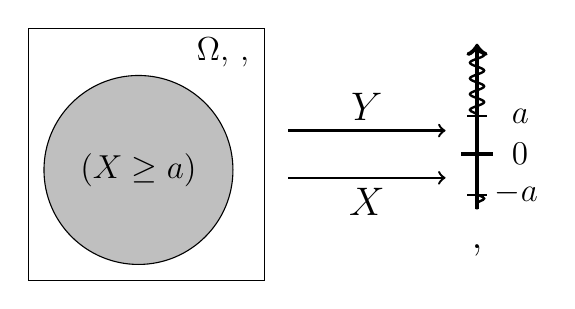
\begin{tikzpicture}
      \begin{scope}
        \fill[lightgray] \firstcircle;
        \draw \drect node[below left] {\large $\Omega, \, \Ac, \, \PP$};
        \draw \firstcircle node {\large $(\abs{X} \geq a)$};
        %Frecce
        \draw[->, line width=0.30mm] (1.8,0.4) node[above,xshift=1cm] {\Large $Y$} -- (3.8, 0.4);
        \draw[->, line width=0.30mm] (1.8,-0.2) node[below,xshift=1cm] {\Large $X$} -- (3.8, -0.2);
        \draw[->, line width=0.60mm] (4.2, -0.6 ) node[below, yshift=-.3cm] {\Large $\RR, \Bc$} -- (4.2, 1.5);
        %Tacchette
        \draw[line width=0.50mm] (4.4, 0.1) node[right, xshift=.1cm] {\large $0$} -- (4, 0.1);
        \draw [|-, line width=0.3mm, decorate,decoration={snake,amplitude=.9mm,segment length=2mm,post length=0mm}] (4.2, -0.4) -- (4.2,-0.6 );
        \draw [|-, line width=0.3mm, decorate,decoration={snake,amplitude=.9mm,segment length=2mm,post length=0mm}] (4.2, 0.6) -- (4.2, 1.5);
        %Scritte
        \node at (4.75, 0.58) {\large $a$};
        \node at (4.7, -0.4) {\large $-a$};
      \end{scope}
    \end{tikzpicture}
    \caption{rappresentazione della VA $Y$}
    \label{img_markov}
  \end{figure}

  Notiamo che $\abs{X(\omega)} \ge Y(\omega) \ \forall \omega$. Abbiamo dunque:
  $$\EE[\abs{X}] \ge \EE[Y] =
  a \cdot \EE\left[\Ind_{(\abs{X}\ge a)}\right] =
  a \cdot 1 \cdot \PP(\abs{X} \ge a)$$
  Dividendo per $a$ si ottiene la tesi.
\end{dimo}

\medskip
\begin{coro}[disuguaglianza di Chebyshev \protect\footnote{In realtà si scrive Čebyšëv e si legge \textit{Ciebiciòff} (Micheletti approves)} \JPTh{9.4}]
  \index{Chebyshev, disuguaglianza di}
  Siano $X$ VAR e un generico valore di soglia $a>0$. Allora:
  $$\PP(\abs{X-\mu}\ge a) \le \frac{Var(X)}{a^2}$$
\end{coro}

La dimostrazione è immediata\footnote{La saprebbe fare anche un gestionale} e segue da Markov prendendo $(X-\mu)^2$ come VA e $a^2$ come valore di soglia. \\
Questa disuguaglianza rivela che la varianza controlla la probabilità che $X$ si allontani dal valore centrale $\mu$ (come peraltro era già stato fatto notare nella sua definizione): più piccola è la varianza, minore è la probabilità (massima) che l'``errore'' di $X$ rispetto a $\mu$ sia superiore a una certa soglia manipolabile arbitrariamente.

\smallskip
\begin{coro}\label{coro-markov}
  Sia $X$ VAR positiva e tale che $\Ex{X} = 0$. Allora $X \aceq 0$.
\end{coro}
\smallskip
\begin{dimo}
  Sia un arbitrario $a > 0$.
  Per la disuguaglianza di Markov $\PP(|X| \geq a) \leq \Ex{|X|}$, con $|X| = X$ per ipotesi.
  Allora $\PP(X \geq a) = 0$.
  La successione di eventi $\left(X \geq \frac{1}{n}\right)$ è crescente, e in particolare $\left(X \geq \frac{1}{n}\right) \uparrow (X > 0)$; pertanto:
  $$\PP\left(X \geq \frac{1}{n}\right) \to \PP(X > 0) = 0
  \implies \PP(X = 0) = 1 \enspace \text{ovvero } X \aceq 0 \qedhere$$
\end{dimo}

\medskip
\begin{corob}[al corollario\footnote{We heard you like corollari so we put a corollario into your corollario}]\label{coro-coro-markov}
  Sia $X \in L^1$ VAR. Allora:
  \begin{align*}
  	\sigma^2 = \Ex{(X-\mu)^2} = 0 & \iff \exists \ c \in \RR \, : \, X \aceq c \\
  	& \iff \exists \ c \, : \, X \sim \delta_c \text{ (delta di Dirac in $c$)}
  \end{align*}
\end{corob}
\smallskip
\begin{dimo}
  \textbf{($\impliedby$)}: Grazie alla regola del valore atteso per le VAR semplici, è noto che $\mu=c$. Si ha quindi che $X-\mu \aceq 0$, ovvero che $(X-\mu)^2 \aceq 0$. 
  Similmente a prima, si conclude che $\sigma^2 = \Ex{(X-\mu)^2} = 0$. \\
  % Quindi $c = \mu$ e $\Ex{(X-\mu)^2} = \EE[X²] - 2\mu \EE[X] + \mu^2 = \mu^2 - \mu^2 = 0$.
  \textbf{($\implies$)}: Poiché $(X-\mu)^2$ è una VAR positiva, per il corollario precedente $(X-\mu)^2 \aceq 0$, ovvero $X \aceq \mu$, dove $\mu$ è il $c$ cercato.
\end{dimo}

\subsection{Valore atteso di serie di variabili aleatorie}
\begin{teob}[\JPTh{9.2}]\label{teo-leibniz-style}
  Sia $\{X_n\}_n$ una successione di VA sullo spazio di probabilità $\Dom$.
  \begin{enumerate}
    \item Se le $X_n$ sono positive, ovvero se $X_n: \Omega \to [0, +\infty]$, allora:
    $$
      \EE\left[\,\sum_{n=1}^{+\infty}X_n \right] = \sum_{n=1}^{+\infty}\EE[X_n] \in [0, +\infty]
    $$
    \item Se $\sum\limits_{n=1}^{+\infty} \EE\big[\abs{X_n}\big] < +\infty$, allora:
    \begin{enumerate}[label=(\roman*)]
      \item $\sum\limits_{n=1}^{+\infty}X_n$ converge quasi certamente;
      \item $\sum\limits_{n=1}^{+\infty} X_n \in L^1$;
      \item $\EE\left[\,\sum\limits_{n=1}^{+\infty} X_n\right] = \sum\limits_{n=1}^{+\infty} \EE[X_n]$.
      \footnote{``Ovvero, siamo nel migliore dei mondi possibili'' -Gottfried von Gregoratti}
    \end{enumerate}
  \end{enumerate}
\end{teob}

\smallskip
\begin{dimo}
  Definiamo le seguenti somme parziali:
  $$S_n \coloneqq \sum_{k=1}^{n}\abs{X_k} \quad \text{e} \quad T_n \coloneqq \sum_{k=1}^{n}X_k$$
  Ne segue, per la linearità (su somme finite) del valore atteso, che:
  $$\EE[S_n] = \EE \left[\,\sum_{k=1}^{n}\abs{X_k}\right] = \sum\limits_{k=1}^{n}\EE\big[\abs{X_k}\big]$$
  Essendo $S_n$ una somma di termini positivi, è crescente e ammette pertanto limite, una VA che chiameremo $S$:
  $$S_n \uparrow S \ \forall \omega, \ \text{con} \ S: \Omega \to [0, +\infty], \ S = \sum_{k=1}^{+\infty}\abs{X_k}$$
  \begin{enumerate}
    \item Se $X_n \ge 0$, la tesi è immediata in quanto $\abs{X_n} = X_n$.
    \item Per ipotesi $\sum\limits_{n=1}^{+\infty} \EE\big[\abs{X_n}\big] < +\infty$.
    Quindi, per dimostrazione precedente, vale anche:
    $$\EE\left[\,\sum_{k=1}^{+\infty}\abs{X_k} \right] = \EE[S] < +\infty
    \implies \PP(S=+\infty) = 0
    \implies \PP(S<+\infty) = 1$$
    In altre parole $S<+\infty$ quasi certamente, che è la tesi (i). \\
    Ora, per la disuguaglianza triangolare si ha che:
    $$ \abs{T_n} = \left\lvert\sum_{k=1}^{n}X_k\right\lvert \le \sum_{k=1}^{n}\abs{X_k} = S_n \ \forall \omega, \forall n$$
    Prendendo i limiti su $n$:
    $$ \abs{T_n} \xrightarrow[n \to +\infty]{\text{qc}} \abs{T} = \left\lvert\sum_{n=1}^{+\infty}X_n\right\lvert \quad \text{e} \quad
    S_n \xrightarrow[n \to +\infty]{\forall \omega} S = \sum_{n=1}^{+\infty} \abs{X_n}$$
    Ne deduciamo che $0 \le \abs{T} \le S$ quasi certamente; per le proprietà del valore atteso con VA positive, vale:
    $$ 0 \le \EE \left[\left\lvert\sum_{n=1}^{+\infty}X_n\right\lvert\right] \le
    \EE\left[\sum_{n=1}^{+\infty}\abs{X_n}\right] < +\infty \quad \text{per ipotesi}$$
    Ne segue che:
    $$ \left\lvert\sum_{n=1}^{+\infty}X_n\right\lvert \in L^1
    \implies \sum_{n=1}^{+\infty}X_n \in L^1$$
    Questo risultato è la tesi (ii).
    Da qui segue anche che:
    $$T_n = \sum_{k=1}^{n}X_k \xrightarrow[n \to +\infty]{\text{qc}} T = \sum_{k=1}^{+\infty}X_k$$
    Poiché $\abs{T_n} \le S_n \le S \in L^1$, per convergenza dominata vale la tesi (iii):
    $$\EE\left[\sum_{n=1}^{+\infty}X_n\right] =
    \lim_{n \to +\infty}\EE[T_n] = \sum_{n=1}^{+\infty} \EE[X_n] \qedhere
    $$
  \end{enumerate}
\end{dimo}

\lezione{12}{04.04.17}
% Parte GG
\subsection{Integrazione di funzioni misurabili}
\begin{teo}[regola del valore atteso \JPTh{9.5}]\label{regola-valore-atteso}
  \index{regola del valore atteso}
  Siano $(\Omega,\Ac, \PP)$ spazio di probabilità, $(F,\Fc)$ spazio misurabile, $X: \Omega \to F $ VA, e $h: F\to \RR$ oppure $[0, +\infty]$ funzione misurabile. Allora:
    \begin{enumerate}
      \item$h(X)\in L^1 \Dom \iff h\in L^1\left(F,\Fc,P^X\right)$
      \item Sia nel caso $h:F\to [0, +\infty]$, sia nel caso $h \in L^1\left(\RR,\Bc,P^X \right)$, si ha:\\
        $$\int_\Omega h(X) \, \dPP = \int_F h \, \de P^X$$
    \end{enumerate}
\end{teo}

Questo teorema è molto importante nel calcolo del valore atteso, perché afferma che svolgere l'integrale su $\Omega$ corrisponde a calcolarlo su $F$.
Infatti, in molti casi il dominio $\Omega$ può essere un insieme astratto composto da oggetti qualsiasi, su cui non è definita l'integrabilità.
\begin{figure}[H]
  \centering
  \def\drect {(-1, -1) rectangle (1, 1)}
  \begin{tikzpicture}
    \draw \drect node[below left] {\large $\Omega, \, \Ac, \, \PP$};
    \begin{scope}[shift={(4cm,0cm)}]
      \draw \drect node[below left] {\large $F, \, \Fc, \, P^X$};
    \end{scope}
    %Frecce
    \draw[->, line width=0.30mm] (1.2,0) node[above,xshift=0.8cm] {\Large $X$} -- (2.6, 0);
    \draw[->, line width=0.30mm] (5.2,0) node[above,xshift=0.8cm] {\Large $h$} -- (6.8, 0);
    \draw[->, line width=0.60mm] (7.2, -0.5) node[below, yshift=-.1cm] {\Large $\RR,\, \Bc,\, P^X$} -- (7.2, 0.8);
    %Tacchette
    \draw[line width=0.50mm] (7.4, 0.0) node[right, align=center] {$\int_F X \de P^X = \int_{\Omega} h(X) \dPP$} -- (7, 0.0);
    %Scritte
  \end{tikzpicture}
  \label{img-regola-valore-atteso-2}
\end{figure}

Imponendo $F = \RR$ il calcolo si trasforma in un integrale su $\RR$, rendendolo possibile o più facile.
Questo è il principale metodo di risoluzione degli esercizi per semplificare i conti. \\
Osserviamo che $\EE$ e $\int_\Omega$ sono la stessa cosa, tuttavia a seconda dei casi una notazione può risultare più comoda rispetto all'altra.
\begin{figure}[H]
  \centering
  \def\drect {(-1, -1) rectangle (1, 1)}
  \begin{tikzpicture}
    \begin{scope}
      \draw \drect node[below left] {\large $\Omega, \, \Ac, \, \PP$};
      %Frecce
      \draw[->, line width=0.30mm] (1.2,0) node[below,xshift=0.8cm] {\Large $X$} -- (2.6, 0);
      \draw[->, line width=0.30mm] (3.5,0) node[below,xshift=2.2cm] {\Large $Y$} -- (7.9, 0);
      \draw[->, line width=0.60mm] (3.2, -0.5) node[below, yshift=-.1cm] {\Large $\RR,\, \Bc,\, P^X$} -- (3.2, 1);
      \draw[->, line width=0.60mm] (8.2, -0.5) node[below, yshift=-.1cm] {\Large $\RR,\, \Bc,\, P^Y$} -- (8.2, 1);
      %Tacchette
      \draw[line width=0.50mm] (3.4, 0.5) node[right] {$\mu = \Ex{X} = \int_{\Omega} X \dPP$} -- (3, 0.5);
      \draw[line width=0.50mm] (8.4, 0.5) node[right] {$\int_\RR X \de P^Y$} -- (8, 0.5);
      %Scritte
    \end{scope}
  \end{tikzpicture}
  \label{img-regola-valore-atteso-1}
\end{figure}

\begin{dimo}
  \Fixvmode
  \begin{enumerate}[label=(\roman*)]
    \item Inizialmente, si prenda per semplicità il caso particolare in cui $h$ è una funzione indicatrice: $h = \Ind_B$, con $B \in \Fc$. Dunque, sfruttando la definizione di controimmagine:
    $$
      \Ind_{B}(X)=\begin{cases}
      1 &\text{per } X(\omega)\in B\\
      0 &\text{per } X(\omega)\notin B
      \end{cases}
      =\begin{cases}
      1 &\text{per } \omega\in(X\in B)\\
      0 &\text{per } \omega\in(X\notin B)
      \end{cases}
      =\Ind_{(X\in B)}(\omega)
    $$
    Da ciò segue che:
    $$
      \int_{\Omega}\Ind_{B}(X)\,\dPP=\int_{\Omega}\Ind_{(X\in B)} \,\dPP =1\cdot\PP(X\in B)=1\cdot P^{X}(B)=\int_{F}\Ind_{B} \,\de P^X
    $$
    Il risultato è la tesi per $h = \Ind_B$.

    \medskip

    \item Prendendo una funzione $h$ semplice, notiamo che è semplice anche la sua composizione:
    $$
      h=\sum_{k=1}^{n}h_{k}\Ind_{B_{k}} \quad \text{con } h_{k}\in\RR, \, B_{k}\in\Fc
    $$
    La dimostrazione si svolge, come nel caso precedente, sfruttando la linearità degli integrali.

    \medskip

    \item Dimostriamo ora la regola nel caso in cui il codominio sia positivo: $h: F \to [0, +\infty]$ misurabile.
    È possibile costruire una successione di funzioni semplici $h_n \geq 0$ tali che $h_n \uparrow h$.
    Questo implica che le $Y_n \coloneqq h_n(X)$ sono VA semplici, che $Y_n \geq 0 \ \forall n$ e che $Y_n \uparrow h(X)$.\\
    Grazie alla convergenza monotona possiamo scambiare integrale e limite e sfruttare la proprietà delle funzioni semplici dimostrata al punto (ii):
    \begin{align*}
      \int_{\Omega}h(x) \, \dPP
      &= \int_{\Omega}\lim\limits_n h_n(X) \, \dPP \;
      \stackrel{\text{cm}}{=} \; \lim\limits_{n}\int_{\Omega}h_{n}(X) \, \dPP \\
      &= \lim\limits_n \int_F h_n \, \de P^X \;
      \stackrel{\text{cm}}{=} \; \int_F \lim\limits_n h_n \, \de P^X
      = \int_F h \, \de P^X
    \end{align*}
    Ma visto che $h \in L^1 (\PP) \iff h\in L^1 \left(P^X\right)$, è evidente che:
    $$\int_\Omega h(x) \dPP = \int_F h \de P^X \quad \forall h:F\to[0, +\infty] \text{ misurabili}$$
    \medskip

    \item Si dimostra ora il caso generale:
    $h\in L^1 \left(P^X\right)$ con $h: F \to \RR$ misurabile.

    Si può separare $h$ nella sua parte positiva $h_{+}$ e negativa $h_{-}$:
    \begin{align*}
      h(X)_+(\omega)
      & =
      \begin{cases}
      h(X) \, (\omega) &\text{per } h(X)(\omega)\geq 0\\
      0     &\text{per } h(X)(\omega) < 0
      \end{cases} \\
      & =
      \begin{cases}
      h( \, X(\omega) \, ) &\text{per } h(X(\omega))\geq 0\\
      0     &\text{per } h(X(\omega)) < 0
      \end{cases}
      \ = h_+(X(\omega))
    \end{align*}
    Analogamente per la parte negativa $h(X)_-(\omega) = h_-(X(\omega))$.\\
    Grazie alla linearità degli integrali possiamo dividere anche questo in parte positiva e negativa:
    $$
      \int_{\Omega}h(x) \,\dPP =
      \int_{\Omega}h(x)_{+} \,\dPP-\int_{\Omega}h(x)_{-} \,\dPP =
      \int_{\Omega}h_{+}(X) \,\dPP-\int_{\Omega}h_{-}(X) \,\dPP
    $$
    Essendo entrambe le funzioni positive, per la dimostrazione al punto (iii):
    $$
      \int_{\Omega}h_{+}(X) \,\dPP-\int_{\Omega}h_{-}(X) \,\dPP =
      \int_{F}h_{+} \,\dP^{X}-\int_{F}h_{-} \,\dP^{X} =
      \int_{F}h \,\dP^X
    $$
    Sfruttando la linearità dell'integrale al contrario otteniamo così la tesi per VA generiche. \qedhere
  \end{enumerate}
\end{dimo}

\medskip

\begin{coro}
  Siano $X$ e $Y$ VA semplici. Allora:
  $$X\aceq Y \implies P^X=P^Y \implies \EE[X]=\EE[Y]$$
\end{coro}
Il corollario amplia il simile risultato che era stato ottenuto per le VA reali: qui $X$ e $Y$ non sono necessariamente reali.

\medskip

\begin{defn}
  \index{valore atteso!su un insieme}
  Dati $X$ VAR e $A \in \Ac$ misurabile, si definisce \textbf{integrale su un insieme} misurabile della VAR la seguente quantità:
  $$\int_A X \, \dPP \coloneqq \int_\Omega X\cdot \Ind_A \, \dPP =  \EE[X \, \Ind_A]$$
\end{defn}
Si noti come nella definizione sia importante la misurabilità di $A$, senza la quale non è possibile definire un'indicatrice misurabile.
Inoltre si può verificare che questa definizione ha senso in quanto la composizione di misurabili è misurabile.

\medskip
\begin{nb}
  La probabilità di un evento $A$ è anche calcolabile con il valore della sua indicatrice:
  $$\PP(A)=\int_{A}1 \, \dPP =\EE[\Ind_{A\\}]$$
\end{nb}

\cleardoublepage
